\documentclass[a4paper]{article}

\usepackage[T1]{fontenc}
\usepackage[utf8]{inputenc}
\usepackage[english]{babel}
\usepackage{fullpage}

\usepackage{amsthm}
\usepackage{amsmath}
\usepackage{amssymb}
\usepackage{textcomp}
\usepackage{stmaryrd}

\usepackage[lastexercise]{exercise}

%\usepackage{graphicx}
%\graphicspath{}

\usepackage{url}

\usepackage[nottoc]{tocbibind}
\usepackage[colorlinks=true,linkcolor=blue]{hyperref}


\newtheorem{Theo}{Theorem}
\newtheorem{Definition}[Theo]{Definition}
\newtheorem{rmk}[Theo]{Remark}
\newtheorem{prop}[Theo]{Property}
\newtheorem{thm}[Theo]{Théorème}
\newtheorem{lm}[Theo]{Lemma}


\newcommand{\sumof}[2]{\underset{#1}{\overset{#2}{\sum}}}
\newcommand{\prodof}[2]{\underset{#1}{\overset{#2}{\prod}}}
\newcommand{\mini}[1]{\underset{#1}{\min}}
\newcommand{\maxi}[1]{\underset{#1}{\max}}
\newcommand{\conj}[1]{\overline{#1}}

\newcommand{\N}{\mathbb{N}}
\newcommand{\Z}{\mathbb{Z}}
\newcommand{\Q}{\mathbb{Q}}
\newcommand{\R}{\mathbb{R}}
\newcommand{\C}{\mathbb{C}}

\renewcommand{\P}{\mathbb{P}}

\usepackage{todonotes}
\newcommand{\oi}[1]{\todo[color=green!40,caption={},size=\tiny]{#1}}
\newcommand{\oii}[1]{\todo[color=green!30,inline]{#1}}

\newcommand\code[1]{{\fontfamily{lmtt}\selectfont #1}}

\title{Directed word with minimal repetition threshold}
\author{Antoine Domenech, Gabrielle Pauvert \& Olivier Idir}
\date{2021-2022}

\newtheorem{theorem}{Theorem}[section]
\theoremstyle{definition}
\newtheorem{definition}{Definition}[section]

\begin{document}

\maketitle

\section{Introduction to the problem}

The goal of this work is to find all pairs $(d, \alpha)$ such that there exists an infinite binary word that is $d$-directed and $(\alpha^+)$-free.

\subsection{Basic notions}

% Let's first define the notions we will work with. 
Let $\Sigma$ and $\Sigma'$ be finite alphabets and $w \in \Sigma^*$. Denote $w = w_1 \dots w_{|w|}$. In practical work, all words will be taken on binary alphabet $\Sigma_2 = \{0,1\}$, or ternary alphabet $\Sigma_3 = \{0,1,2\}$.

\begin{definition}{\textbf{Directedness:}}
%A word $w = w_1w_2...w_n$ over an alphabet $A$ 
$w$ 
is said to be $d$-directed if, for all factor $u$ of $w$ of size $d$, say $u = w_iw_{i+1}...w_{i+d-1}$, its reversed sequence $u^T = w_{i+d-1}w_{i+d-2}...w_i$ is not a factor of $w$.
\end{definition}

\begin{definition}{\textbf{Freeness:}}

Let $w$ a word over alphabet $\Sigma$. A factor of $w$ is called a repetition if it is of shape $(uv)^nu$, where $u \in \Sigma^*, v \in \Sigma^+, n \in \N^*$. We call $|(uv)^nu|$ the length of the repetition, $|u|+|v|$ the period of the repetition, and $\frac{|(uv)^nu|}{|u|+|v|} = n + \frac{|u|}{|u| + |v|}$ the size of the repetition.

$w$ is said to be $\alpha$-free (resp. $\alpha^+$-free) if it has no factor that is a repetition of size greater or equal to (resp. strictly greater than) $\alpha$.

%A word $w$ over alphabet $A$ is said to be $\alpha$-free if it does not contain any repetition of size $\alpha$ or more, i.e. there are no factors of the shape $u_1v_1u_2v_2...u_n v_n u_{n+1}$ where $n \ge 1$, $\forall i \in \{1,...,n+1\}, u_i = u_1$, $\forall i \in \{1,...,n\}, v_i = v_1$, such that : $n + \frac{|u_1|}{|u_1| + |v_1|} \ge \alpha$.\oii{Si on a l'égalité des $u_i$, pourquoi ne pas le mettre dès le départ de la forme "$uvuvuvu$ with $n+1$ occurences of $u$ (thus $n$ of $v$)" ? --> on peut, d'ailleurs on peut aussi écrire u...uv avec v préfixe de u. J'ai hésité entre tous ces trucs.}

%We call $|u_1| + |v_1|$ the period of the repetition, and $n + \frac{|u_1|}{|u_1| + |v_1|}$ its size (not to be confounded with its length).

%A word $w$ over alphabet $A$ is said to be $(\alpha^+)$-free if it does not contain any repetition of size strictly greater than $\alpha$, but repetitions of size exactly alpha are allowed.
\end{definition}

\begin{definition}{\textbf{Uniform and Synchronizing:}}
Let $q\in \N^+$. A morphism $\phi : \Sigma \mapsto \Sigma'$ is said to be $q$-uniform if the image of every letter in $\Sigma$ has length $q$.

If $\phi$ is $q$-uniform, $\phi$ is said to be synchronizing if for all letter $a_1, _a2, a_3 \in \Sigma$, the image $\phi(a_1)$ is a factor of  $\phi(a_2)\phi(a_3)$ if and only if it's a prefix or a suffix of that concatenation.
\end{definition}

\subsection{Defining the problem}

Observe that if $\beta \ge \alpha$ and $w$ is $\alpha$-free, then $w$ is also $\beta$-free. Indeed, any repetition in $w$ is of size at most $\alpha$, thus it is of size lower than $\beta$. Similarly, observe that if a word $w$ is $\alpha$-free, then it is also $(\alpha^+)$-free, but the converse is not true. Take $\alpha$ the exact maximum size of a repetition in $w$ (of the form described in Definition 1.1.) then $w$ is $(\alpha^+)$-free but not $\alpha$-free.
% This is called the repetition threshold. -> Nope ^^

Thus, the existence of a $(\alpha^+)$-free infinite word entails the existence of infinite $\beta$-free words for any $\beta \ge \alpha$. As a consequence, to find all pairs $(d, \alpha)$ such that there exists an infinite binary word that is $d$-directed and $(\alpha^+)$-free, we can focus on finding the $\alpha$ that is tight for each $d$. That is to say, find the unique $\alpha$ such that there exists an infinite $d$-directed $(\alpha^+)$-free word, but there exist no $d$-directed $\alpha$-free word.

Now a similar observation can be made with directedness. If $d' \ge d$ and $w$ is $d$-directed, then $w$ is also $d'$-directed. Indeed, look at the converse. If a factor of size $d'$ has its reverse in $w$, then take the prefix of this factor of size $d$, its reverse is a factor of $w$.

Thus, for a given $\alpha$, to prove that there are infinite $d$-directed $(\alpha^+)$-free words, it is enough to focus on the minimal $d$ that ensures this existence.

%\section{Initial construction via backtracking}

%Initially, being quite unfamiliar with this notion, we first implemented an algorithm able to find, for a given tuple $(d, \alpha, l)$, a word $d$-directed and $(\alpha^+)$-free 

\section{Algorithm outline and main results}

\subsection{Finding tight alpha values}
\label{alpha}

A computer can be used to search by backtracking for a $d$-directed $(\alpha^+)$-free (or $\alpha$-free) word of size $l$, for given $d$, $\alpha$ and $l$. The code written for this purpose will be explained in details in section \ref{code}. 

Whenever the backtrack ends without finding such a word, then since the computer enumerated all words satisfying these two conditions in the process, we can be sure that there are no such word of size $l$, and thus no such infinite word. Indeed, if there were an infinite word, its prefix of size $l$ would still be $d$-directed and $(\alpha^+)/\alpha$-free.

However, when the computer finds a large word (say $l$ = 1000 for example) during the backtracking, then we can conjecture that an infinite $d$-directed and $(\alpha^+)/\alpha$-free word exists.

Using this algorithm, we can conjecture the values of tight alpha for every small value of $d$, by running a dichotomy on $\alpha \in \mathcal{Q}$ for each $d$. Search between $2$ (the Repetition Threshold bound on binary alphabet) and $3$, for example. We will then prove them to be indeed tight in \ref{morphism}. 

\subsection{Results}
\label{results}

Here are the results of the dichotomies :

\begin{center}
\begin{tabular}{ | c || c | c | c | c | c | c | c | c | c | c | c |}
\hline
 $d$ & 5 & 6 & 7 & 8 & 9 & 10 & 11 & 12 & 13 & 14 & ... \\ 
\hline
 $\alpha$ & $\infty$ & 3 & 3 & 8/3 & 8/3 & 5/2 & 5/2 & 5/2 & 7/3 & 7/3 & ... 7/3 ... \\
\hline
\end{tabular}
\end{center}

\paragraph{}

Note that in this table, the lower bounds for the values $\alpha$ are already proven (except for $d$ = 5). The backtracking ended without finding any $\alpha$-free $d$-directed word, so we know that infinite such words don't exists, thus tight $\alpha$ is at least the value given in the table.

To prove that $\alpha$ is exactly the value given above, we still need the upper bound. We will reach these $\alpha$ by generating infinite words that are $d$-directed and $(\alpha^+)$-free for these values. Recall by observations made in \ref{alpha} that we need only to generate infinite words for the couples $(6,3)$, $(8,8/3)$, $(10,5/2)$ and $(13,7/3)$. The generated words will also be $d$-directed and $(\alpha^+)$-free for the same value of $\alpha$ and bigger $d$.

\paragraph{}

This will leave us with two more things to prove, stated here as a conjecture :
\begin{itemize}
\item There are no $5$-directed $\alpha$-free word for any $\alpha \in \mathcal{R}^+$. Enumerating them by backtracking points out that every 5-directed word of size $l$ large (say $l \ge 100$ for example) is made of a repetition of either "101100" or its complementary "010011" if we ignore the border effects (constraints are easier to satisfy on the sides of the word).
\item For all $d \ge 13$, there are no $d$-directed $7/3$-free infinite words. Computer check was made up to $d = 250$.
\end{itemize}

The theoretical study of these results goes beyond the work of this paper.

	% TODO : lister les couples d, alpha
	% morphismes !
	% présenter le code et ses optims
	
	
\section{Generating infinite words}
\label{morphism}

\subsection{Theoretical result}	
	
	%Cette secton adapte le lemme 2.1 de \href{https://www.lirmm.fr/~ochem/morphisms/OchemTIA.pdf}{cet %article}.
	
	%\begin{thm} Let $\alpha, \beta \in \Q, 1 < \alpha < 2 < \beta < 3$ and $n \in \N$. Let $h:\Sigma_3^* %\rightarrow \Sigma_2^*$ be a synchronizing q-uniform morphism ($q \geq 1$). If for every %$\alpha^+$-free finite word $w$ such that $|w| < \max \left( \frac{TOCOPY}{\beta -\alpha}, TOCOPY %\right)$ h(w) is $\beta^+$-free, then for every $\alpha^+$-free infinite word $t$, $h(t)$ is %$\beta^+$-free.
	%\end{thm}
	%\begin{proof}
	%Assume there is a $w$ is an $\alpha^+$-free word such that $h(w)$ is not $\beta^+$-free, and consider %a $w$ of minimal length for this property. Thus $h(w)$ contains a $\beta^+$ repetition : a factor %$uvuvu$ such that $\frac{|uvuvu|}{|uv|} > \beta$. Denote $x = |u|$ and $y = |v|$, so %$\frac{3x+2y}{x+y}$, hence $y < x\frac{3-\beta}{\beta-2}$. Let's distinguish two cases : 
	%\begin{itemize}
	%    \item If $x \geq 2q-1$ 
	%    \item 
	%\end{itemize}
	%\end{proof}
	% preuve adaptée ? -> généraliser à n < alpha < m < o ?


This section adapts lemma 2.1 from \cite{lemma}. For this project, we need to take $\beta = \frac{7}{3} > 2$, which is not covered by the lemma, hence the need to reprove following result :
	
\begin{theorem}
\label{thm}
Let $\alpha, \beta \in \Q$, $1 < \alpha < \beta < 3$  with $2 < \beta$ and $n \in \N$. Let $h:\Sigma_s^* \rightarrow \Sigma_e^*$ be a synchronizing q-uniform morphism (with $q \geq 1$). If for every $\alpha^+$-free word $w$ such that $|w| < \max \left( \frac{2\beta}{\beta - \alpha}, \frac{2(q-1)(3\beta - 4)}{q(\beta - 2)} \right)$ $h(w)$ is $\beta^+$-free, then for every (finite or infinite) $\alpha^+$-free word $t$, $h(t)$ is $\beta^+$-free.
\end{theorem}
\begin{proof}
Assume for contradiction that there is a $w$ is an $\alpha^+$-free word such that $h(w)$ is not $\beta^+$-free, and consider a $w$ of minimal length with this property. Thus $h(w)$ contains a $\beta^+$ repetition, that is, a factor $uvuvu$ such that $\frac{|uvuvu|}{|uv|} > \beta$. Denote $x = |u|$ and $y = |v|$. Since $\frac{|uvuvu|}{|uv|} = \frac{3x+2y}{x+y} > \beta$, we have :
%\\
$y < \frac{3-\beta}{\beta-2}x$ (1). Let's distinguish two cases : 

\begin{itemize}

\item If $x \geq 2q-1$, then each occurrence of $u$ contains at least one full $h$-image of a letter. As $h$ is synchronizing, the two occurrences of $u$ in $uvu$ contain the same h-images and in the same positions. Let $U$ be the factor of $w$ that contains all letters whose $h$-images are fully contained in $u$, so that $h(U)$ is a factor of u which only misses at most $q-1$ letters at each side of $u$. Let $V$ be the factor of $w$ that contains all letters whose $h$-images intersect $v$, so that $h(V)$ contains $v$ as a factor, along with at most $q-1$ letters at each side.

Denoting $X = |U|$ and $Y = |V|$, we then have $Yq < y + 2q$ and $Xq > x - 2q$, or equivalently $x < (X + 2)q$ (2). Since $UVUVU$ is a factor of $w$ and $w$ is $\alpha^+$-free, then $\frac{3X+2Y}{X+Y} \le \alpha$. Remark that if $\alpha < 2$, we already have a contradiction.

From above inequality we deduce that $X \le \frac{\alpha-2}{3-\alpha}Y$ (3). Now we have :

$$ Yq < y + 2q <_{(1)} \frac{3-\beta}{\beta-2}x + 2q <_{(2)} \frac{3-\beta}{\beta-2}(X+2)q + 2q $$
$$ <_{(3)} \frac{3-\beta}{\beta-2}( \frac{\alpha-2}{3-\alpha}Y +2)q + 2q $$

implying that $ Y < \dfrac{2(3-\alpha)}{\beta- \alpha}$ (4).

By the minimality of $w$, we need to add at most one letter at both side of $UVUVU$ to get $w$ (such that $h(w)$ covers $uvuvu$). Thus we get :

$$ |w| \le 2 + 2Y + 3X \le_{(3)} 2 + Y(2 + 3\frac{\alpha-2}{3-\alpha}) <_{(4)} 2 + \dfrac{2(3-\alpha)}{\beta- \alpha}(2 + 3\frac{\alpha-2}{3-\alpha}) = \frac{2\beta}{\beta - \alpha}. $$

This contradicts the hypothesis verified by the morphism.

\item Else $x \leq 2q-2$, then by (1) we get $y < \frac{3-\beta}{\beta-2}(2q-2)$ and thus $3x + 2y \le \frac{2\beta}{\beta - 2}(q-1)$. Using minimality of $w$ like above and uniformity of the morphism, we get that $(|w| - 2)q \le |uvuvu| - 2 = 3x + 2y - 2$. By the previous inequality, we deduce $|w| < \frac{2(q-1)}{q}\frac{3\beta - 4}{\beta - 2}$.

Again, this contradicts the hypothesis verified by the morphism.

\end{itemize}
\end{proof}

\subsection{Application and computer search}

Now we will apply Theorem \ref{thm} with $\alpha = 7/4$ (the minimal value for which an infinite ternary $\alpha^+$-word exists), and $\beta$ the value for which we want to generate an infinite binary $\beta^+$-free word, i.e. $\beta$ takes values in $\{3,8/3,5/2,7/3\}$.

A computer can be used once again to search for morphisms $\phi$ satisfying the conditions of Theorem \ref{thm}. The search follows additional conditions to preserve $d$-directedness : Denote $L$ the set of all factors of size $d$ contained in the concatenation of the images of any two different letters. Then we must have that $L$ does not contain a word $u$ and its reverse $u^T$\oi{Attention, dans la nouvelle déf le reverse s'appelle $u^T$}. For example, for all factors $u$ in $\phi(0)\phi(1)$, $u^T$ must not appear in $\phi(2)\phi(0)$ (or any other concatenation). Also $q$ must be greater than $d$. 

This backtracking is much heavier and will be explained in the code section.

\paragraph{}

Here are the minimal morphisms found (with regard to $q$) :

\begin{itemize}
    \item ($d,\alpha) = (6,3)$, $q = 13$ :
\begin{align*}
  & 0 \longmapsto 0101100101110\\
\phi_6 : \hspace{1cm} & 1 \longmapsto 0101100010110 \\
  & 2 \longmapsto 0010101110001
\end{align*}
    \item ($d,\alpha) = (8,8/3)$, $q = 30$ :
    \begin{align*}
  & 0 \longmapsto 011001001011001001011011001011\\
\phi_8 : \hspace{1cm} & 1 \longmapsto 001001011011001011011001001011 \\
  & 2 \longmapsto 001001011011001001011011001011
\end{align*}
    \item ($d,\alpha) = (10,5/2)$, $q = 26$ :
    \begin{align*}
  & 0 \longmapsto 00101001011010110010110011\\
\phi_{10} : \hspace{1cm} & 1 \longmapsto 00101001011001100101101011 \\
  & 2 \longmapsto 00101001011001011010110011
\end{align*}
\item ($d,\alpha) = (13,7/3)$, $q = 62$ :
    \begin{align*}
  & 0 \longmapsto 00110110010011001011010010110011011001011001001100101101001011\\
\hspace{-1.25cm} \phi_{13} : \hspace{1cm} & 1 \longmapsto 00110110010011001011010010110010011001011001101100101101001011 \\
  & 2 \longmapsto 00100110010110011011001001100101101001011001001100101101001011
\end{align*}
\end{itemize}

These morphisms are respectively 13-uniform, 30-uniform, 26-uniform and 62-uniform. We have $1 < 7/4 < \alpha < 3$ and $2 < \alpha$ for all above $\alpha$ values. Additional checks by computer ensure that $\phi_6$, $\phi_8$, $\phi_{10}$ and $\phi_{13}$ are synchronizing and that the images of every $7/4^+$-free ternary words of maximal size given by the theorem are $\alpha^+$-free.

Moreover, it is known that there exists an infinite ternary $7/4^+$- free word (and even that this is the repetition threshold for ternary word, i.e. the best repetition size we can achieve)\cite{ternary}. Thus, the images of such a word by the $\phi$ morphisms are infinite $\alpha^+$-free binary words.

Also, since any $7/4^+$-free ternary word $w$ is in particular $2$-free, i.e it is square-free, we know it doesn't have any factor of the form $aa$ where $a$ is a letter. Thus, since $q \ge d$, every factor of size $d$ in $\phi(w)$ is either contained in the image of a letter $\phi(a)$ or intersecting the image of two letters $\phi(a_1)\phi(a_2)$ with $a_1 \neq a_2$. So, by property of $\phi$, we know that $\phi(w)$ is $d$-directed, a factor of size $d$ and its reverse cannot simultaneously appear in $\phi(w)$.

This concludes in the existence of $d$-directed $\alpha^+$-free words for every couple $(d,\alpha)$ given above. The finite $\alpha$ values given in \ref{results} are tight.

Remark : The Thue Morse ternary sequence is not $7/4^+$-free, but its image by these morphisms seems to be $d$-directed $\alpha^+$-free still.


\section{Algorithmic details}
\label{code}
%Explain the OCaml code in detail.

This section is a guide to the code used in this article. It explains the algorithmic ideas used to perform the searches and verifications mentioned above. For the technical implementations, see the readmes, and the code files with their own documentations and comments.

\subsection{Directedness}

For generating a $d$-directed word by backtracking, the idea is to store all factors of size $d$ of the word we are constructing in a binary tree. A left child represents a 0, and a right child represents a 1.

\begin{figure}[ht]
\centering
  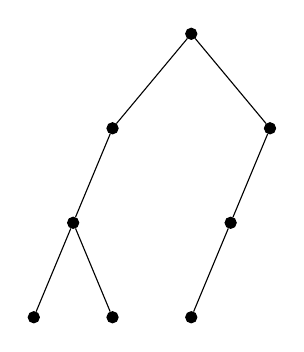
\begin{tikzpicture}[level distance=12mm]
  \tikzstyle{every node}=[circle,inner sep=0.05cm, fill = black]
  \tikzstyle{level 1}=[sibling distance=20mm]
  \tikzstyle{level 2}=[sibling distance=20mm]
  \tikzstyle{level 2}=[sibling distance=10mm]
  \node[circle,draw, fill = black]{}
     child {node[circle,draw]{}
       child {node[circle,draw] {}
         child {node[circle,draw] {}}
         child {node[circle,draw] {}}
       }
       child[missing]
     }
     %child[missing]
     child {node[circle,draw] {}
        child {node[circle,draw]{}
            child {node[circle,draw]{}
            }
            child[missing]
        }
        child[missing]
     }
     ;
	\end{tikzpicture}
	 \caption{Tree of factors containing 000, 001 and 100}
    \label{fig:exemple}
\end{figure}

%This is much more efficient than, say, a list of factors for example. Indeed, if $w$ contains the factors 000 and 001, the second factor only adds one child in the tree. Search and adds in the tree are linear in $d$.

Now for every letter we add to the word, if the letter forms a new factor (i.e. the word we are generating has reached size $d$ at least), we add this factor to the tree and we check that the reverse of this factor is not in the tree. If it is in the tree, we go back in the backtracking, otherwise we can go on to the next letter. 

Note : if the factor is a palindrome then it is its own reverse so the reverse is indeed in the tree (since we just added it).

\paragraph{}
The tree of factors is similarly used for the $d$-directedness test. We read the tested word letter by letter, and for each of them we add to the tree the factor of size $d$ ending at this letter, then we check that its reverse is not in the tree.

\subsection{Freeness}

To ensure that the generated word in the backtracking is $\alpha(^+)$-free, we check that adding a letter at the end of the word preserves $\alpha(^+)$-freeness. To do that, we verify that every suffix of the word, i.e every new factor added to the word, is not a repetition of size (strictly) greater than $\alpha$. 

In practice, if we add letter $w_n$ at the end of word $w=w_1w_2...w_{n-1}$, for every $p \ge 1$, we compute the longest repetition with period of size $p$ ending on the last letter $w_n$. This is of size 0 if $w_{n-p} \neq w_{n}$, else we move on to check if $w_{n-p-1} = w_{n-1}$, etc. Denote $i$ the first index at which letters differ (it can be n-p, or 0 if the beginning of the word is reached). $w_{i+1}w_{i+2}...w_{n}$ is a repetition of period $p$ and of repetition size $\frac{w_{i+1}w_{i+2}...w_{n}}{p} = \frac{n-i}{p}$ (see definition of freeness for this formula). We take the maximum over all the repetition sizes we found, and check that it is (strictly) lower than $\alpha$.

Note that we only need to check period sizes up to $\left\lfloor \frac{n}{\alpha} \right\rfloor$ since a bigger period would not allow to fit enough repetition of the period in the word to exceed $\alpha$ repetition size.

To test if a word is $\alpha(^+)$-free, we read it letter by letter and check that each of them preserved $\alpha(^+)$-freeness.

\subsection{Morphism Generation}

Generating a morphism is a little more complex than generating a word, since we have to find three words (the images of 0, 1 and 2) satisfying many more conditions. To do this, we generate all three images of same size $q$ at once by generating a $d$-directed $\alpha(^+)$-free word of size $3q$. That way we already cover two of the possible concatenations of images. Now we have to check all the other concatenations.

Say we are generating word $W = W_1W_2W_3$ where $W_1$, $W_2$ and $W_3$ are words of size $q$. When we reach the letter at positions $2q$, i.e. end of $W_2$, we have to check concatenation of $W_2$ with $W_1$. That is, we add to the tree of factors all words of size $d$ that are a concatenation of a suffix of $W_2$ and a prefix of $W_1$, and check that their reverses are not in the tree. Run a loop over such factors beginning at letters $(W_2)_{q-d+i+1}$ for $i$ varying from $1$ to $d-1$.

To that end and for a later use, we keep track of the suffix of $W_1$ and the prefixes and $W_1$ and $W_2$ of size $d$ in new separate variables.

Now when we reach the beginning of $W_3$, say the $i-th$ letter of $W_3$, we similarly need to test all factors from concatenation of a suffix of $W_1$ and a prefix of $W_3$. Since we are building these prefixes along the way, we can add-check $(W_1)_{q-d+i+1}...(W_1)_q(W_3)_1...(W_3)_i$ for all $i$ between 1 and $d-1$ while we generate letter $(W_3)_i$.

Finally, when we reach the end of $W_3$, we have to add-check all factors of size $d$ that are concatenations of a suffix of $W_3$ with a prefix of $W_1$ or $W_2$.
%\oii{Partie pas très claire de manière générale, il n'y a pas moyen de dire quelque chose de style "$\forall i,j \in [1;2;3]$, we add-check the factors at the junction $W_iW_j$" ? (après avoir add-check les facteurs internes) -> non, car justement on teste au fur et à mesure (ce que cette partie explique) et non uniuement à la fin +1}

We also check that the images we generated for 0, 1 and 2 are all different.

\paragraph{}

As for $\alpha(^+)$-freeness, we want that all the images of square-free ternary words are $\alpha^+$-free. Thus, we must have that any concatenation of square-free images is also $\alpha^+$-free, so we add some checks when reaching the end of $W_2$ and $W_3$. In the first case, we test freeness of $W_2W_1$, and in the second case we test every square-free concatenation of three images. While this is not proven to be enough for the hypothesis of theorem \ref{thm}, it still gives a pretty strong candidate that will be proven to satisfy $\alpha^+$-freeness of every image of $(7/4^+)$-free ternary word later on.\\
This last function is also a backtracking enumerating all ternary $(7/4)^+$-free words and testing $\alpha^+$-freeness of their images.

The synchronizing condition is also tested afterward.

\subsection{Dichotomy}

The dichotomy to find tight $\alpha$ for a given $d$ is made on rational numbers instead of floats since we are hoping to get the exact values of tight alpha. Instead of taking the mean between minimum $\alpha_{min} = \frac{p}{q}$ and maximum $\alpha_{max} = \frac{p'}{q'}$ we can take as intermediate value $\alpha_{inter} = \frac{p+p'}{q+q'}$ to have a lower growth of denominator and less need for reducing fractions.

\bibliographystyle{unsrt}
\bibliography{bibli}

\end{document}